\documentclass[mathserif,serif]{beamer}
\usepackage{tabularx}
\setbeamertemplate{footline}[frame number]
% \useoutertheme{infolines}
\usepackage{slidesphysics}
\graphicspath{{../plot/}}

\title[]{Data/MC comparison}
\author[]
{
Samuel Lo \inst{1}
\and
Yanjun Tu  \inst{1}
\and
Dongliang Zhang  \inst{2}
}
\institute[]
{
\inst{1}
The University of Hong Kong
\and
\inst{2}
University of Michigan
}
\date[]{\today}

\newcommand\Wider[2][3em]{%
\makebox[\linewidth][c]{%
\begin{minipage}{\dimexpr\textwidth+#1\relax}
\raggedright
\centering#2
\end{minipage}%
}%
}

\begin{document}
\frame{\titlepage}

\begin{frame}{Introduction}
\begin{itemize}
\item Check the charge flip BG in the pre-selection level.
\item Use old charge flip rate by Gabriel.
\item Replace Z+jets and single-top by charge flip BG.
\item Define SS\_ee Control Region:
\begin{itemize}
\item $|m_{ll}-m_Z| < 10$ GeV
\end{itemize}
\item The $m_{ll}$ plot is a N-1 plot.
\end{itemize}
\end{frame}

\begin{frame}{Expected number of events \\ For CR\_nonISR\_SS\_ee\_Zmass}
\vspace{5mm}
\begin{tabular}{|c|c|c|}
\hline
& Number of events & Significance \\
\hline
VV & $87.6\pm2.3$ & \\
\hline
V$+\gamma$ & $179.7\pm10.2$ & \\
\hline
fake lepton & $1437.8\pm23.0$ & \\
\hline
charge flip & $14585.1\pm4.7$ & \\
\hline
Total BG & $16290.2\pm25.7$ & \\
\hline
Data & $15164.0$ & \\
\hline
Signal (400, 380) & $0.5\pm0.1$ &\\
\hline
Signal (400, 350) & $3.1\pm0.3$ &\\
\hline
Signal (400, 300) & $1.8\pm0.2$ &\\
\hline
Signal (400, 200) & $0.8\pm0.2$ &\\
\hline
Signal (400, 100) & $0.9\pm0.2$ &\\
\hline

\end{tabular}
\end{frame}

\begin{frame}{Expected number of events \\ For CR\_ISR\_SS\_ee\_Zmass}
\vspace{5mm}
\begin{tabular}{|c|c|c|}
\hline
& Number of events & Significance \\
\hline
VV & $51.3\pm1.5$ & \\
\hline
V$+\gamma$ & $37.4\pm4.3$ & \\
\hline
charge flip & $2335.7\pm2.8$ & \\
\hline
fake lepton & $394.8\pm12.1$ & \\
\hline
Total BG & $2819.1\pm13.2$ & \\
\hline
Data & $2612.0$ & \\
\hline
Signal (400, 380) & $0.1\pm0.0$ &\\
\hline
Signal (400, 350) & $1.2\pm0.1$ &\\
\hline
Signal (400, 300) & $1.0\pm0.2$ &\\
\hline
Signal (400, 200) & $0.2\pm0.1$ &\\
\hline
Signal (400, 100) & $0.2\pm0.1$ &\\
\hline

\end{tabular}
\end{frame}


\begin{frame}{For CR\_SS\_ee\_Zmass \\ $p_T^{l1}$}
\Wider{
\includegraphics[width=0.8\textwidth]{pt1_CR_SS_ee_Zmass}
}
\end{frame}

\begin{frame}{For CR\_SS\_ee\_Zmass \\ $p_T^{l2}$}
\Wider{
\includegraphics[width=0.8\textwidth]{pt2_CR_SS_ee_Zmass}
}
\end{frame}

\begin{frame}{For CR\_SS\_ee\_Zmass \\ $\eta^{l1}$}
\Wider{
\includegraphics[width=0.8\textwidth]{eta1_CR_SS_ee_Zmass}
}
\end{frame}

\begin{frame}{For CR\_SS\_ee\_Zmass \\ $\eta^{l2}$}
\Wider{
\includegraphics[width=0.8\textwidth]{eta2_CR_SS_ee_Zmass}
}
\end{frame}

\begin{frame}{For CR\_SS\_ee\_Zmass \\ $\phi^{l1}$}
\Wider{
\includegraphics[width=0.8\textwidth]{phi1_CR_SS_ee_Zmass}
}
\end{frame}

\begin{frame}{For CR\_SS\_ee\_Zmass \\ $m_{ll}$}
\Wider{
\includegraphics[width=0.8\textwidth]{mll_CR_SS_ee_Zmass}
}
\end{frame}

\begin{frame}{For CR\_SS\_ee\_Zmass \\ $p_T^{ll}$}
\Wider{
\includegraphics[width=0.8\textwidth]{ptll_CR_SS_ee_Zmass}
}
\end{frame}

\begin{frame}{For CR\_SS\_ee\_Zmass \\ $E_{\text{T}}^{\text{miss}}$}
\Wider{
\includegraphics[width=0.8\textwidth]{MET_CR_SS_ee_Zmass}
}
\end{frame}

\begin{frame}{For CR\_SS\_ee\_Zmass \\ $m_{T2}$}
\Wider{
\includegraphics[width=0.8\textwidth]{mTtwo_CR_SS_ee_Zmass}
}
\end{frame}

\begin{frame}{For CR\_SS\_ee\_Zmass \\ $m_{\text{T}}^{l1}$}
\Wider{
\includegraphics[width=0.8\textwidth]{mt1_CR_SS_ee_Zmass}
}
\end{frame}

\begin{frame}{For CR\_SS\_ee\_Zmass \\ $m_{\text{T}}^{l2}$}
\Wider{
\includegraphics[width=0.8\textwidth]{mt2_CR_SS_ee_Zmass}
}
\end{frame}

\begin{frame}{For CR\_SS\_ee\_Zmass \\ $p_T$ of the leading jet}
\Wider{
\includegraphics[width=0.8\textwidth]{jetpt_CR_SS_ee_Zmass}
}
\end{frame}

\begin{frame}{For CR\_SS\_ee\_Zmass \\ $\eta$ of the leading jet}
\Wider{
\includegraphics[width=0.8\textwidth]{jeteta_CR_SS_ee_Zmass}
}
\end{frame}

\begin{frame}{For CR\_SS\_ee\_Zmass \\ Number of jets}
\Wider{
\includegraphics[width=0.8\textwidth]{nJet_CR_SS_ee_Zmass}
}
\end{frame}

\begin{frame}{For CR\_SS\_ee\_Zmass \\ Number of b-jets}
\Wider{
\includegraphics[width=0.8\textwidth]{nBJet_CR_SS_ee_Zmass}
}
\end{frame}

\begin{frame}{For CR\_SS\_ee\_Zmass \\ Number of central jets}
\Wider{
\includegraphics[width=0.8\textwidth]{nCJet_CR_SS_ee_Zmass}
}
\end{frame}

\begin{frame}{For CR\_SS\_ee\_Zmass \\ $|\Delta\phi_{ll}|$}
\Wider{
\includegraphics[width=0.8\textwidth]{l12_dPhi_CR_SS_ee_Zmass}
}
\end{frame}

\begin{frame}{For CR\_SS\_ee\_Zmass \\ $|\Delta\phi_{ll,\text{MET}}|$}
\Wider{
\includegraphics[width=0.8\textwidth]{l12_MET_dPhi_CR_SS_ee_Zmass}
}
\end{frame}

\begin{frame}{For CR\_SS\_ee\_Zmass \\ $|\Delta\phi_{\text{jet0,MET}}|$}
\Wider{
\includegraphics[width=0.8\textwidth]{jet0_MET_dPhi_CR_SS_ee_Zmass}
}
\end{frame}

\begin{frame}{For CR\_SS\_ee\_Zmass \\ $|\Delta\eta_{ll}|$}
\Wider{
\includegraphics[width=0.8\textwidth]{dEta_CR_SS_ee_Zmass}
}
\end{frame}

\begin{frame}{For CR\_SS\_ee\_Zmass \\ $E_{\text{T}}^{\text{miss,rel}}$}
\Wider{
\includegraphics[width=0.8\textwidth]{METRel_CR_SS_ee_Zmass}
}
\end{frame}

\begin{frame}{For CR\_SS\_ee\_Zmass \\ $m_{\text{eff}}$}
\Wider{
\includegraphics[width=0.8\textwidth]{meff_CR_SS_ee_Zmass}
}
\end{frame}

\begin{frame}{For CR\_SS\_ee\_Zmass \\ $m_{\text{T}}^{\text{max}}$}
\Wider{
\includegraphics[width=0.8\textwidth]{mtm_CR_SS_ee_Zmass}
}
\end{frame}

\begin{frame}{For CR\_SS\_ee\_Zmass \\ $m_{lj}$/$m_{ljj}$}
\Wider{
\includegraphics[width=0.8\textwidth]{mlj_CR_SS_ee_Zmass}
}
\end{frame}

\begin{frame}{For CR\_SS\_ee\_Zmass \\ $m_{jj}$}
\Wider{
\includegraphics[width=0.8\textwidth]{mjj_CR_SS_ee_Zmass}
}
\end{frame}



\section{Conclusion}
\begin{frame}{Conclusion}
\begin{itemize}
\item The agreement is not good.
\item maybe I need to apply trigger requirement.
\end{itemize}
\end{frame}

\section{Plan}
\begin{frame}{Plan}
\begin{itemize}
\item Use charge flip tagger to estimate charge flip BG.
\end{itemize}
\end{frame}

\begin{frame}
\begin{center}
\huge
Backup
\end{center}
\end{frame}

\begin{frame}[fragile]
\frametitle{Signal sample}
\small
Sample Name(p2972 tag):
\tiny
\begin{verbatim}
mc15_13TeV.993820.MGPy8EG_A14N13LO_C1N2_Wh_2L_175_0.merge.DAOD_SUSY2.e5678_a766_a821_r7676_p2949_p2972
mc15_13TeV.993821.MGPy8EG_A14N13LO_C1N2_Wh_2L_165_35.merge.DAOD_SUSY2.e5678_a766_a821_r7676_p2949_p2972
mc15_13TeV.993822.MGPy8EG_A14N13LO_C1N2_Wh_2L_400_0.merge.DAOD_SUSY2.e5678_a766_a821_r7676_p2949_p2972
\end{verbatim}
\end{frame}

\begin{frame}[fragile]
\frametitle{Data}
\small
use both 2015 and 2016 data (3212.96 + 32861.6) /pb
\tiny
\begin{verbatim}
GRL:
GoodRunsLists/data16_13TeV/20161101/physics_25ns_20.7.xml
GoodRunsLists/data15_13TeV/20160720/physics_25ns_20.7.xml
\end{verbatim}
\end{frame}

\begin{frame}{MC BG}
p-tag: p2949
\end{frame}

\begin{frame}[fragile]
\small
Trigger list:\\
\scriptsize
\begin{verbatim}
2015
HLT_2e12_lhloose_L12EM10VH
HLT_e17_lhloose_mu14
HLT_mu18_mu8noL1

2016(A-D3)
HLT_2e17_lhvloose_nod0
HLT_e17_lhloose_nod0_mu14
HLT_mu20_mu8noL1

2016(D3-)
HLT_2e17_lhvloose_nod0
HLT_e17_lhloose_nod0_mu14
HLT_mu22_mu8noL1
\end{verbatim}
\end{frame}

\begin{frame}{Object Definitions}
\small
Tool: AnalysisBase 2.4.31, SUSYTools-00-08-60\\

\centering
\begin{table}
\small
\begin{tabularx}{\textwidth}{p{1.5cm} | p{3cm} | p{3cm} | p{3cm}}
& \textbf{Electron} & \textbf{Muon} & \textbf{Jet}\\
\hline
\textbf{Baseline}
& - $p_T>10$ GeV \newline - $|\eta^{cluster}| < 2.47$ \newline - LooseAndBLayerLLH
& - $p_T>10$ GeV \newline - $|\eta| < 2.7$ \newline - Medium
& - $p_T>20$ GeV \\
\hline
\textbf{Signal}
& - $p_T > 25$ GeV \newline - $|\eta^{cluster}| < 2.47$ \newline - TightLLH \newline - GradientLoose \newline - $|z_0 \sin \theta| < 0.5$mm \newline - $|d_0/\sigma_{d_0}| < 5$
& - $p_T > 25$ GeV \newline - $|\eta| < 2.7$ \newline - Medium \newline - GradientLoose \newline - $|z_0 \sin \theta| < 0.5$mm \newline - $|d_0/\sigma_{d_0}| < 3$
& - $p_T > 20$ GeV \newline - $|\eta|<2.8$ \newline \newline - $|JVT| > 0.59$ \newline if $p_T < 60$ GeV \newline and $|\eta| < 2.4$
\end{tabularx}
\end{table}

\raggedright
Selection:
\begin{itemize}
%\item Trigger selection
\item Exactly 2 baseline leptons and exactly 2 signal leptons
\end{itemize}

\tiny
Note: \\
Pileup reweighting is applied. \\
Scale factor for reconstruction, isolation, ID and trigger is applied.
\end{frame}

\begin{frame}
\frametitle{averageMu}
\begin{figure}
\includegraphics[width=0.33\textwidth]{averageMu_CR_ISR_OS_ee}
\includegraphics[width=0.33\textwidth]{averageMu_CR_ISR_OS_mumu}
\includegraphics[width=0.33\textwidth]{averageMu_CR_ISR_OS_emu} \\
\caption{Average number of interactions per bunch crossing, for ee channel (left), $\mu\mu$ channel (middle) and e$\mu$ channel (right).}
\end{figure}
\end{frame}

\begin{frame}
\frametitle{Definition of jets}
\normalsize
\begin{itemize}
\item Central jets: $\pt>20$ GeV, $|\eta|<2.4$, no b-tagged
\begin{itemize}
\item This is the run 1 definition.
\end{itemize}
\item B-jets: b-tagged
\end{itemize}
\end{frame}

\begin{frame}
\frametitle{significance calculation}
\begin{itemize}
\item RooStats::NumberCountingUtils::BinomialExpZ(S,B,$\delta$B)
\item $\delta$B = sqrt((0.25)\^{}2 + (nBGError/nBG)\^{}2)
\begin{itemize}
\item use the same definition from Dani.
\end{itemize}
\end{itemize}
\end{frame}

\begin{frame}
\frametitle{definition of variables}
\normalsize
\begin{itemize}
\item HT: Sum of the $p_T$ of all signal jets and the two leptons.
\item R2 = MET / (MET + pt1 + pt2)
\item l12\_dPhi: difference in phi between the two leptons.
\item l12\_MET\_dPhi: difference in phi between MET and the sum of 4-momentum of the two leptons.
\end{itemize}
\end{frame}

\begin{frame}
\small
SUSY scenario:\\
\begin{figure}
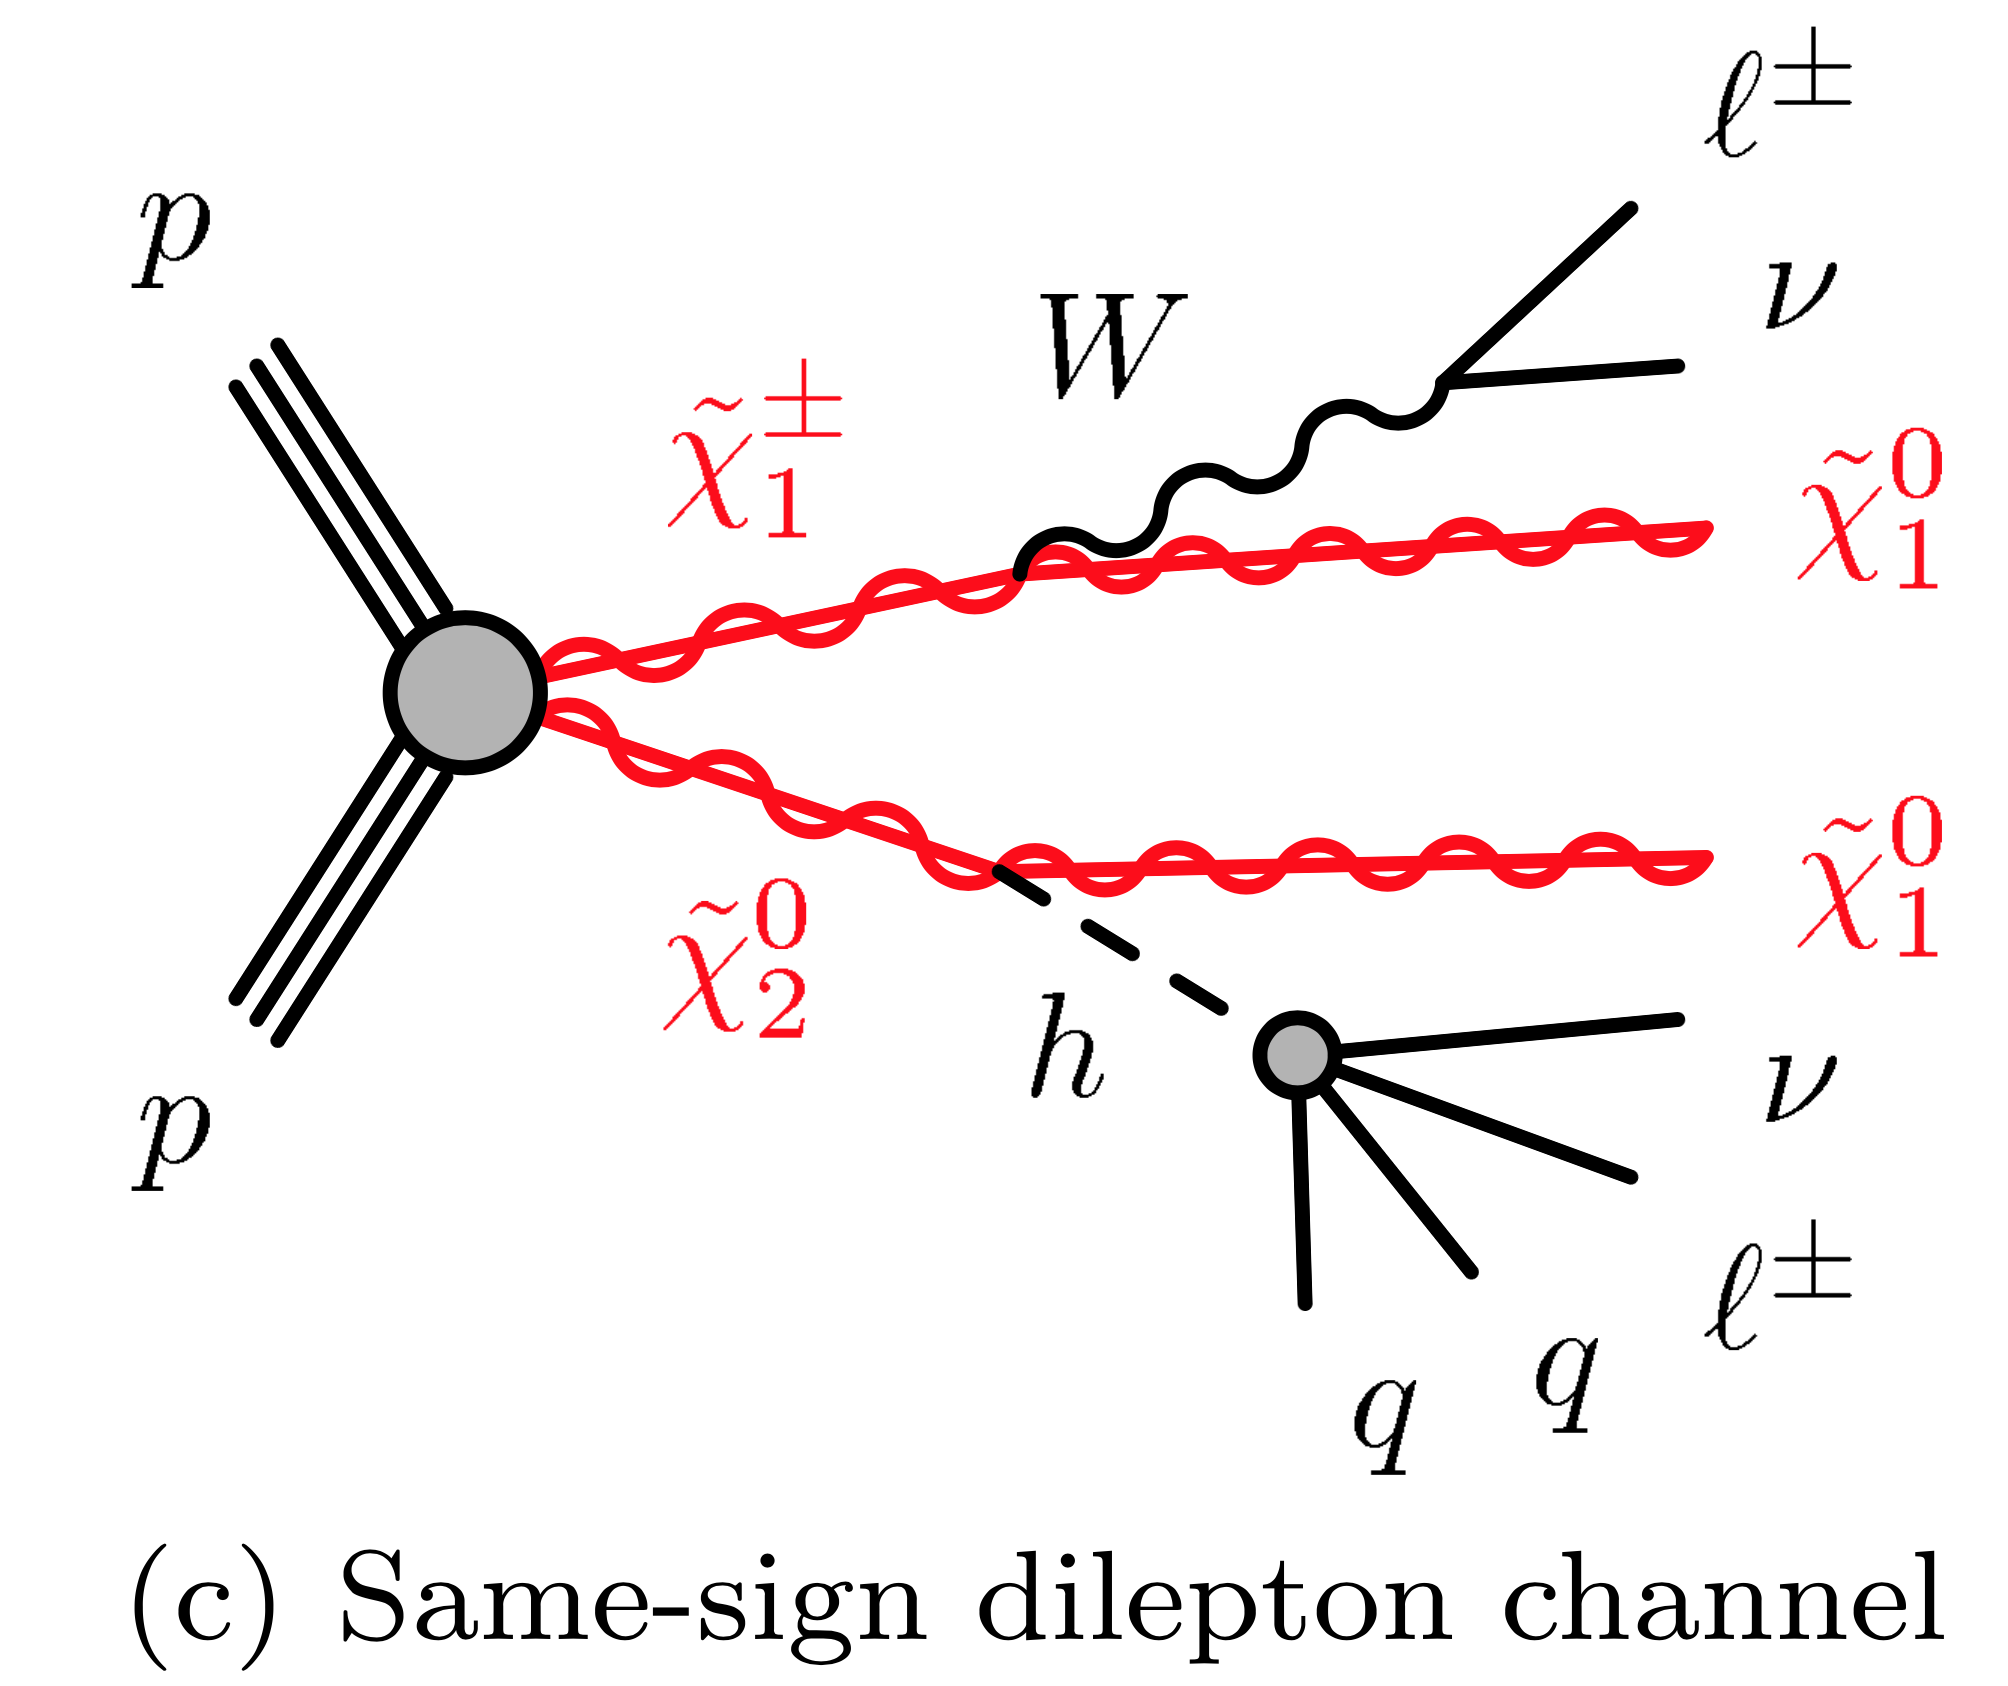
\includegraphics[width=0.6\textwidth]{data/photo/Wh.png}
\end{figure}
\end{frame}

\begin{frame}{Selection in run1 SR}
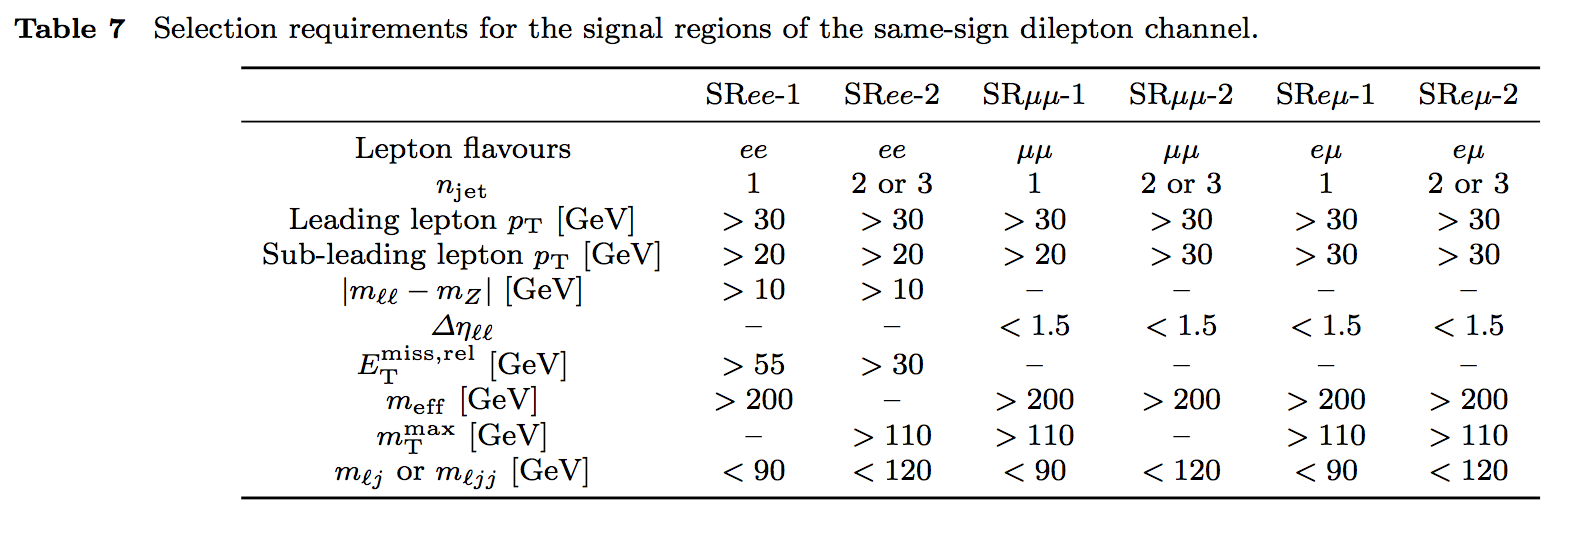
\includegraphics[width=\textwidth]{data/photo/SRcutrun1.png} \\
\url{https://arxiv.org/pdf/1501.07110.pdf}
\end{frame}
\end{document}
